\chapter{Opis informatyczny}
\label{appx:opis_informatyczny}

\section*{Model programowy}

Na rysunku \ref{fig:gmm_diagram} przedstawiono zależności pomiędzy poszczególnymi klasami w implementacji algorytmu \textit{GMM}. Z kolei rysunek \ref{fig:vibe_pbas_diagram} pokazuje architekturę i funkcję zaimplementowane w algorytmach \textit{ViBE} oraz \textit{PBAS}. Wyszczególniono najistotniejsze komponenty, zarówno te o dostępie publicznym (poprzedzone znakiem +), jak i prywatnym (poprzedzone znakiem -). 

		\begin{figure}[h!]
				\centering
				%\includegraphics[width=\textwidth,height=18cm,keepaspectratio = false]{dodatki/FTSG_diagram.png}
				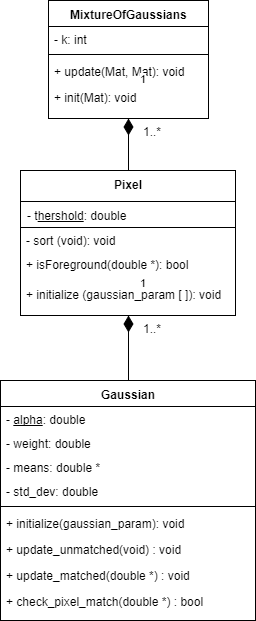
\includegraphics[scale = 0.6]{img/appx/gmm_architecture.png}
				\caption{Diagram zależności pomiędzy klasami -- algorytm \textit{GMM}}
				\label{fig:gmm_diagram}
		\end{figure}
		
		\begin{figure}[h!]
				\centering
				%\includegraphics[width=\textwidth,height=18cm,keepaspectratio = false]{dodatki/FTSG_diagram.png}
				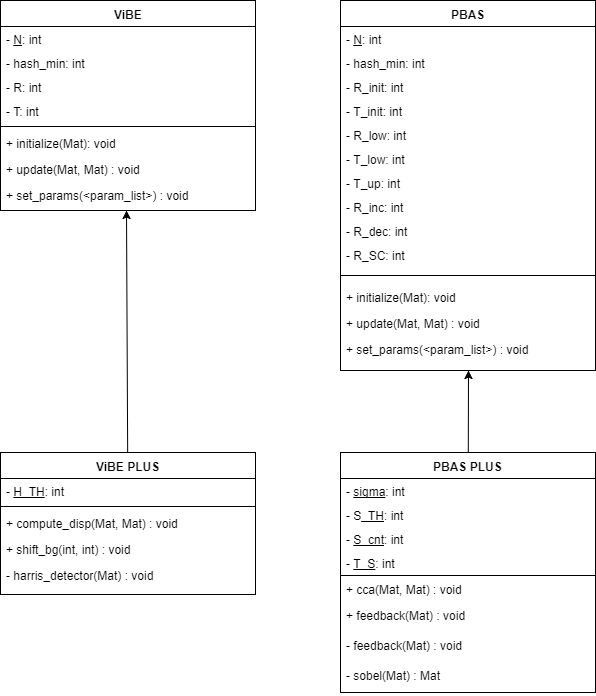
\includegraphics[scale = 0.6]{img/appx/vibe_pbas_architecture.png}
				\caption{Diagram zależności pomiędzy klasami -- algorytmy \textit{ViBE} i \textit{PBAS}}
				\label{fig:vibe_pbas_diagram}
		\end{figure}

\section*{Projekty w środowisku Vivado}

\paragraph*{Moduły użyte w algorytmie \textit{ViBE}}

\begin{eqwhere}[5cm]
    \item[\textit{harrisEdge.v}] moduł realizujący detekcję narożników metodą Harrisa-Stephensa
    \item[\textit{medianHistogram.v}] moduł obliczający medianę z zebranych próbek
    \item[\textit{model\_3d\_update.v}] moduł aktualizujący sąsiednie modele tła
    \item[\textit{model\_update.v}] moduł aktualizujący model tła
    \item[\textit{pad\_crop.v}] moduł realizujący przesunięcie modelu tła    
    \item[\textit{pixel\_match\_test\_cielab.v}] moduł realizujący test dopasowania
    \item[\textit{rgb2cielab.v}] konwersja do przestrzeni \textit{CIELab}
    \item[\textit{update\_arbitrator.v}] moduł decydujący o dokonaniu aktualizacji
    \item[\textit{vibe\_cielab.v}] moduł realizujący algorytm \textit{ViBE} w przestrzeni \textit{CIELab}
    \item[\textit{vibe\_cielab\_init.v}] moduł inicjalizujący model tła
    \item[\textit{vibe\_plus.v}] moduł realizujący rozszerzony algorytm \textit{ViBE}
    \item[\textit{visualize.v}] moduł wizualizujący przepływ optyczny
\end{eqwhere}

\paragraph*{Moduły użyte w algorytmie \textit{PBAS}}

\begin{eqwhere}[5cm]
    \item[\textit{cca.v}] moduł analizujący obiekty statyczne
    \item[\textit{cfd.v}] moduł realizujący odejmowanie dwóch kolejnych ramek
    \item[\textit{decision\_thr.v}] moduł aktualizujący próg decyzji
    \item[\textit{feedback\_ctrl.v}] moduł realizujący pętlę sprzężenia zwrotnego
    \item[\textit{labeller.v}] moduł realizujący indeksację jednoprzebiegową    
    \item[\textit{learning\_rate.v}] moduł aktualizujący współczynnik uczenia
    \item[\textit{model\_3d\_update.v}] moduł aktualizujący sąsiednie modele tła    
    \item[\textit{model\_update.v}] moduł aktualizujący model tła    
    \item[\textit{pbas\_1c.v}] moduł realizujący algorytm dla jednej składowej	    
    \item[\textit{pbas\_rand\_init.v}] moduł inicjalizujący model tła    
    \item[\textit{pbas\_rgbs.v}] moduł realizujący algorytm \textit{PBAS} w przestrzeni \textit{RGB}  
    \item[\textit{pbas\_plus\_rgbs.v}] moduł realizujący rozszerzony algorytm \textit{PBAS}   
    \item[\textit{pbas\_gray.v}] moduł realizujący algorytm \textit{PBAS} w skali szarości
    \item[\textit{pixel\_match\_test\_1c.v}] moduł realizujący test dopasowania dla jednej składowej
    \item[\textit{update\_arbitrator.v}] moduł decydujący o dokonaniu aktualizacji	
    \item[\textit{updateEdgeSimMeasure.v}] moduł aktualizujący parametr $S_{O_k}$	
    \item[\textit{updateStaticObjectHistory.v}] moduł aktualizujący parametr $EC_{O_k}$
\end{eqwhere}


\paragraph*{Pozostałe moduły}
\begin{eqwhere}[4.5cm]
    \item[\textit{context\_3x3.v}] moduł generujący kontekst o rozmiarze 3x3
	\item[\textit{delay\_line\_bram\_wp.v}] linia opóźniająca zrealizowana z wykorzystaniem pamięci \textit{BRAM}	
	\item[\textit{delay\_x\_x.v}] linia opóźniająca
	\item[\textit{median\_9x9.v}] filtr medianowy 9x9
	\item[\textit{mem\_ctrl.v}] kontroler pamięci RAM
	\item[\textit{moving\_avg.v}] moduł realizujący algorytm średniej kroczącej
	\item[\textit{naive\_method.v}] moduł realizujący metodę naiwną
	\item[\textit{rgb2gray.v}] moduł realizujący konwersję do skali szarości
	\item[\textit{rng\_128.vhd}] generator liczb pseudolosowych
	\item[\textit{subtract.v}] moduł realizujący odejmowanie ramek
\end{eqwhere}

\paragraph*{Lista plików realizujących algorytm \textit{GMM}} -- źródło \cite{piszczek_15}
\begin{itemize}[noitemsep, topsep=0pt]
	\item \textit{background\_classifier.v}
	\item \textit{comparator.v}
	\item \textit{gaussian\_updater.v}
	\item \textit{match\_condition.v}
	\item \textit{match\_found\_updater.v}
	\item \textit{match\_tester.v}
	\item \textit{model\_updater.v}
	\item \textit{no\_match\_found\_updater.v}
	\item \textit{sorter.v}
\end{itemize}